\documentclass[letterpaper,12pt, titlepage]{article}

\usepackage[spanish]{babel}
\usepackage[utf8]{inputenc}

\usepackage{graphicx}
\usepackage{tabularx}
\usepackage{slashbox}
\usepackage[intlimits]{amsmath}
\usepackage{amssymb}
%\usepackage[left=2cm, right=2cm, top=4cm, bottom=3.5cm]{geometry}

\DeclareGraphicsExtensions{.jpg,.pdf,.mps,.png,.eps}

\newcommand{\ms}{\texttt}

\begin{document}

\title{	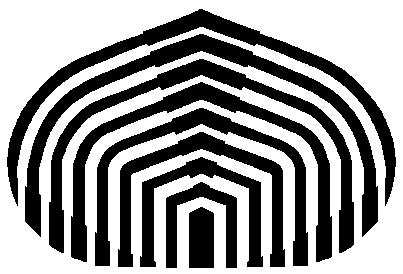
\includegraphics[height=80pt]{usb.jpg} \\
CI-5437 \\ Inteligencia Artificial I \\
Proyecto I\\
Búsqueda}
\author{Kelwin Fernández y Alejandro Machado\\
	Universidad Simón Bolívar} 
\date{Junio de 2010} 
\maketitle

\section{Decisiones de implementación}

\subsection{Representación de Perfiles}

Para la representación explícita de un perfil optamos por
implementarlos compactando las preferencias que representen
la misma permutación de candidatos, de esta forma cada permutación
$a_0, a_1, \ldots, a_n$ de estos aparecerá a lo sumo una vez
en un perfil. En cada perfil, las preferencias se encuentran
almacenadas en un vector de forma ordenada.

Todo esto garantiza que cada perfil esté unívocamente representado
independientemente de con que cambios elementales hemos llegado
hasta él, evitando así la repetición de estados.

\bigskip
Se establece adicionalmente una relación de orden sobre perfiles,
$\sqsubseteq$, determinada por el orden lexicográfico de sus
preferencias, más adelante se explicará el uso de esta relación
de orden.

\subsection{Representación de Estados}

Dadas las consideraciones impuestas sobre elespacio de búsqueda,
tenemos que podemos considerar un \textit{branching factor} de a
lo sumo $m\cdot(n-1)$, donde $m$ es el número de electores y $n$
el número de candidatos. Aunado a esto tenemos un número máximo
de candidatos de $250$, considerando que tenemos $10^6$ de electores
obtendremos un \textit{branching factor} máximo de $249\times 10^6$.
Si consideramos a un estado del espacio de búsqueda como el perfil
completo, al ejecutar una cambio elemental en el algoritmo de
búsqueda en amplitud habremos de mantener en memoria $55$
\textit{petabytes}.

Todo apunta a mantener el mínimo número posible de perfiles en
memoria y optar por una representación compacta para los estados.

\subsubsection*{BFS}

En el caso de BFS, dada la forma de su recorrido, el número de
nodos crecerá exponencialmente, por lo que una representación
compacta permitirá ahorrar recursos para que el algoritmo pueda
concluir su ejecución, en ciertos casos, sin agotar la memoria
del computador.

En lugar de almacenar un perfil completo, para cada estado
se guarda cuál fue el último cambio elemental realizado (cuál
candidato, en cuál preferencia), y un apuntador al estado padre.

Es necesario mantener una lista de estados ``cerrados" (ya
generados por el algoritmo) para una correcta implementación
de búsqueda en amplitud. En este caso, los estados visitados
se mantuvieron en un vector ordenado mediante la siguiente
relación de orden sobre Estados:

Sean $a, b$ estados generados por el algoritmo de búsqueda en
profundidad:

$$a \prec b \equiv f(a) < f(b) \ \vee \ (f(a) = f(b) \ \wedge \ Perfil(a) \sqsubseteq Perfil(b))$$

Donde $f$ es una función de clasificación asociada a los
estados y $Perfil(a)$ es el perfil generado por el estado
$a$. El valor de la función de clasificación para cada estado 
es precalculado al generarlo y se obtiene de forma semejante
a la función heurística heurística sugerida para el algoritmo
IDA*. Dando un orden $a_0, a_1, \ldots, a_n$ sobre los candidato,
tenemos que la función de clasificación de un estado $s$ viene
dada por:

$$f(s) = \Sigma_{i\in [0..n]} (b^i\cdot T'(a_i))$$

\hspace*{-0.5cm}donde $b$ es una constante que dispersa los
resultados de cada $T'(a_i)$ para evitar colisiones y que en
nuestro caso obtuvimos mejor resultados con $b=10$.

\bigskip
La intuición detrás de esta decisión es la siguiente:
dos estados que evalúan a un diferente valor de la función de clasificación
deben ser distintos, y por lo tanto no hay que obtener los perfiles asociados
y compararlos, lo cual consume tiempo. En algunos casos, una búsqueda binaria
sobre el vector de nodos visitados puede arrojar el resultado que se necesita
sin tener que obtener ningún perfil.

Adicionalmente se almacena la profundidad de cada estado, a fin de no
seguir expandiendo fronteras del último nivel si ya se ha hallado una
solución en éste.

\subsubsection*{IDA*}

Para este algoritmo se utilizó un solo perfil. Cuando vamos a expandir
un nodo, consideramos uno de sus sucesores, aplicamos un cambio elemental
y llamamos recursivamente a su sucesor. Una vez que el sucesor devuelve
una respuesta, se desaplica el cambio elemental, se expande sistemáticamente
hacia el próximo hijo y así sucesivamente hasta agotar los posibles cambios
elementales. 

De esta forma se reduce la memoria utilizada de $b\cdot d$ a $d$, donde
$b$ es el \textit{branching factor} y $d$ la longitud de camino. Cada
vez que expandimos un nodo no generamos inmediatamente todos sus
sucesores, generamos uno a uno y vamos explorando por cada uno de 

La lista de estados visitados se representa con un protocolo $LIFO$ que
permita simular las llamadas recursivas. En esta lista se presentan los
continuos cambios que se han venido aplicando para, de esta forma, poder
construir desde el estado inicial cada uno de los nodos intermedios.

\section{Obtención de sucesores}
\subsubsection*{BFS}
    Para obtener los sucesores de un estado, debe construirse primero
    el perfil asociado y luego aplicar todos los posibles cambios elementales
    sobre éste.

\subsubsection*{IDA*}
    Se aplica un cambio elemental sobre
    el perfil actual, y se explora el perfil hijo. Posteriormente,
    se deshace este cambio elemental; este proceso se repite para
   cada transición posible.

\section{Optimizaciones}

\subsubsection*{General}
    \begin{enumerate}
       \item Agregar un votante a una preferencia existente dentro de un perfil
       es $O(log(n))$, donde $n$ es el número de preferencias. Esto se logra
       manteniendo las preferencias ordenadas dentro de cada perfil.
    \end{enumerate}

\subsection*{BFS}
    \begin{enumerate}
       \item Los estados generados se mantienen en un vector ordenado,
       lo que garantiza, al utilizar búsqueda binaria, que a lo sumo
       se realizará un número logarítmico (en el número de estados
       generados) de comparaciones para determinar si se debe generar un
       nuevo estado.

		\item Se mantienen en memoria dos perfiles. Uno con el perfil
		actual y otro con el padre de la iteración anterior. Dado el
		recorrido que realiza la búsqueda en profundidad, $b-1$ nodos
		de la frontera utilizarán el padre que generó su hermano, evitando
		así el cálculo adicional de generar cada perfil desde el inicial.
		
		\item Se guarda el nivel de profundidad para no expandir nodos más
		allá de una meta.
		
		\item Gracias a la función de clasificación se evita generar
		cada perfil del vector de estados generados. Más adelante se
		muestran ciertos resultados acerca de la proporción de mejora
		de esta función.

		\item Los nodos generados se almacenan en un vector ordenados
		bajo la relación de orden dada para los estados, permitiendo
		así una búsqueda logarítmica.
\end{enumerate}

\subsection*{IDA*}

\begin{enumerate}
\item Al no verificar repeticiones sobre el espacio de búsqueda,
los tiempos de ejecución del algoritmo de IDA* mejoran considerablemente,
por lo tanto se consideró una opción adicional que permite correr el
algoritmo sin verificar repeticiones.
\end{enumerate}

\section{Opciones añadidas}

\begin{itemize}
\item \ms{-prop}: Imprime en cada intento de generar un nuevo estado
la proporción de comparaciones resueltas utilizando la función de
clasificación.

\item \ms{-nomem}: Permite ejecutar el algoritmo IDA* sin verificar
estados repetidos.

\end{itemize}

\section{Discusión de resultados}
Mejor no memorizar
\section{Recomendaciones}
Permutation ranking
\end{document}
